\documentclass[12pt,letterpaper]{article}
\usepackage[utf8]{inputenc}
\usepackage[english]{babel}
\usepackage{amsmath}
\usepackage{amsfonts}
\usepackage{amssymb}
\usepackage{graphicx}
\usepackage{caption}
\usepackage{subcaption}
\usepackage[capposition=top]{floatrow}
\usepackage[left=2cm,right=2cm,top=2cm,bottom=2cm]{geometry}
\author{White Team \\ Chenxi Rong, Xiaoquan Liu, Zhanyi Lin, Fabian Schmid}
\title{Estimate the Impact of Opioid Control Policies \\ (Report for Policy Maker)}
\begin{document}
\maketitle

\section*{Executive Summary}

The higher numbers of opioids, both prescribed and illegally used, cause severe problems in the United States like increasing overdose deaths. For that reason, several states introduced legislation to counter this trend. To analyze the effectiveness of such policies, this report summarizes the evidence of interventions in Florida, Texas, and Washington. 

We used opioid shipment data published by the Washington Post and drug overdose death data by the US Vital Statistics records for each county and year to implement two common statistical approaches. We compared the trend before and after the policy went into effect in each state. In addition, we compared this trend with the trend in similar states to get more robust results. These approaches show heterogeneity in the magnitude of the effects between states and between the analyzed outcome. 

Our results imply that Florida's and Texas' drug policy decreased both the prescription opioid shipment amount and the overdose deaths. In contrast, Washington's approach was only successful in lowering the growth rate in overdose deaths.

\section{Motivation}
According to the Centers for Disease Control and Prevention (CDC), the number of drug overdose deaths has quintupled since 1999. The rise in opioid overdose deaths can be outlined in three distinct waves: the first wave in the 1990s with increased prescribing of opioids, the second wave in 2010 with heroin, and the third wave in 2013 with synthetic opioids like fentanyl. In order to fight the opioid overdose epidemic, policymakers have made policy interventions to limit the over prescription of opioids. Texas regulations with regard to treating pain with controlled substances went into effect in January 2007. Florida's legislature became effective in 2010, and a series of changes related to drug prescription took place in the following years. Washington regulated the prescribing requirements of opioids for pain treatment in January 2012, which included periodic patient reviews, milligram thresholds, strict documentation guidelines, and consultations with pain management experts.

For all three of these policy changes, we performed both a pre-post analysis and a difference-in-difference analysis to understand the effect of opioid drug regulations on both the amount of opioid shipments and drug overdose deaths. For the pre-post analysis, we will demonstrate the trend of overdose deaths and opioid shipments over years. After the policy went into effect, we analyze if our plots show a difference in the trend in each state right before the policy became effective and right after it. To further valid our analysis, we conduct a difference-in-difference analysis. We look at the development in the state with a policy change over time and compare it to the trend in similar states which are not affected by the policy.

We used drug overdose death data from the US Vital Statistics records, prescription opioid drug shipments from the Washington Post, and US census population data. One strength of the analysis is that it is based on a large number of observations and credible data sources. However, we cannot evaluate the effects on overdose deaths in counties with less than 10 overdose deaths per year. Due to privacy reason this data is not available and can potential bias our results by a small margin. Two different approaches and two different outcomes variables are analyzed to get detailed insights on the effects of opioid regulations. Only for the policy change in Texas in 2007, limited opioid shipment data is available for the time before the policy implementation. To assess the validity of our analysis, it is important to know that the pre-post and the diff-in-diff analysis both rely on crucial assumptions to evaluate the policies sufficiently. For the pre-post analysis, we have to assume that no other event took place at the same time of the policy implementation which might also affect the overdose deaths or the shipped opioids. This might be violated if the US Customs Service managed to dramatically reduce the importation of fentanyl into the United States at the same time Florida's policy went into effect. This would likely reduce the number of overdose deaths throughout the United States. The diff-in-diff analysis is more flexible but still requires to assume that the state with a policy change and the states without a policy change behave similarly if no policy would have been implemented. For that reason, we picked three states with similar trends prior to the policy implementation to compare with. These assumptions have to be taken into account, when reading through the following analysis. 

\section{Analysis}
\subsection{Florida}

\textbf{Opioid shipments}

\begin{figure}[!h]
\centering
\begin{subfigure}{.5\textwidth}
  \centering
  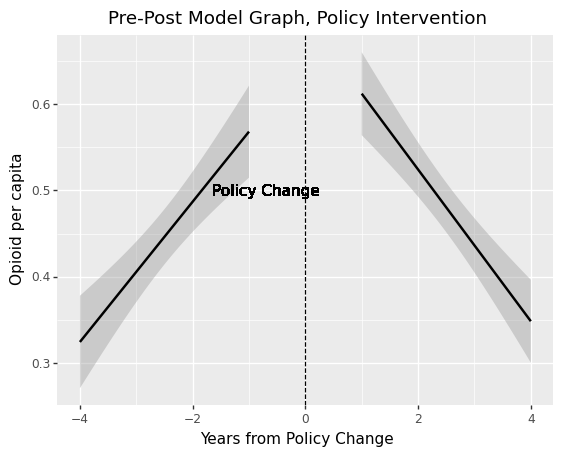
\includegraphics[width=.7\linewidth]{../30_results/General_Results/florida_opioid_shipment_prepost.png}
  \caption{Pre-post analysis}
  \label{fig:fl_ship_prepost}
\end{subfigure}%
\begin{subfigure}{.55\textwidth}
  \centering
  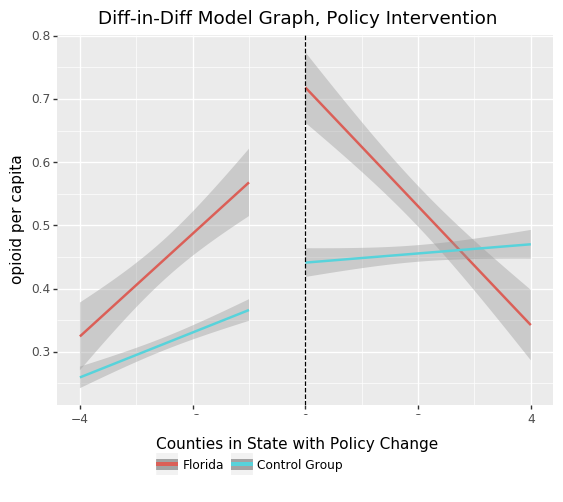
\includegraphics[width=1\linewidth]{../30_results/General_Results/florida_opioid_shipment_diffdiff.png}
  \caption{Diff-in-diff analysis}
  \label{fig:fl_ship_did}
\end{subfigure}
\caption{Analysis of opioid policy on opioid shipments in Florida}
\floatfoot{\textit{Note:} The control group includes Tennessee, West Virginia, and Nevada. The shipped opioids per capita are measured in grams and converted to morphine equivalents. The lines are the linear trend before and after the policy change. The shaded area indicates the range we expect our estimates to fall in with a 95\% level of confidence.}
\label{fig:fl_ship}
\end{figure}

In the left graph in Figure \ref{fig:fl_ship}, we can see an increasing trend in opioid shipments per capita which reverses after the policy is introduced. In the right graph, we compared the development of opioid shipments in Florida with the one in Tennessee, West Virginia, and Nevada. The output shows that in the states without a policy change, the number of shipped opioids per capita is still increasing over time while the opioid shipments in Florida decrease. Therefore, we may conclude that the decrease of opioid shipments per capita in Florida after 2010 is caused by the policy, which implies that the policy is effective. \\

\noindent \textbf{Overdose deaths} \\

\begin{figure}[!h]
\centering
\begin{subfigure}{.5\textwidth}
  \centering
  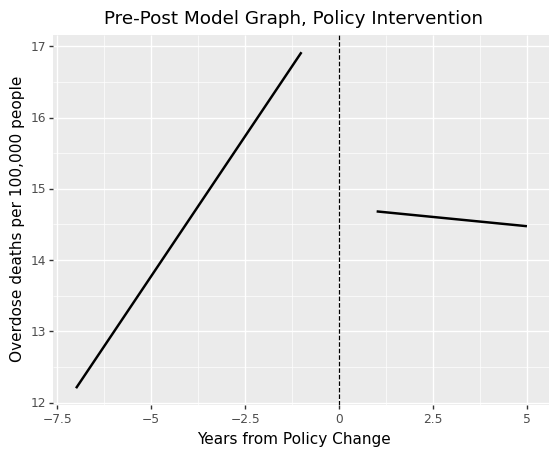
\includegraphics[width=0.7\linewidth]{../30_results/General_Results/florida_overdose_death_prepost.png}
  \caption{Pre-post analysis}
  \label{fig:fl_death_prepost}
\end{subfigure}%
\begin{subfigure}{.55\textwidth}
  \centering
  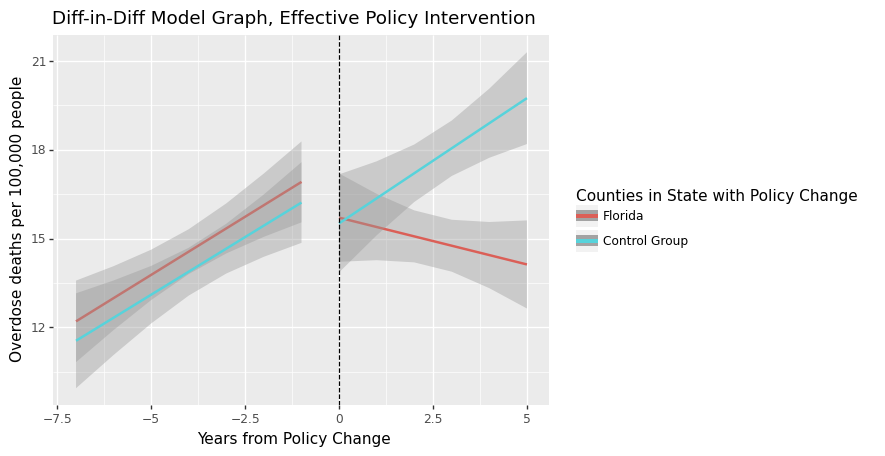
\includegraphics[width=1\linewidth]{../30_results/General_Results/florida_overdose_death_diffdiff.png}
  \caption{Diff-in-diff analysis}
  \label{fig:fl_death_did}
\end{subfigure}
\caption{Analysis of opioid policy on overdose deaths in Florida}
\floatfoot{\textit{Note:} The control group includes North Carolina, Tennessee, and Iowa. The lines are the linear trend before and after the policy change. The shaded area indicates the range we expect our estimates to fall in with a 95\% level of confidence.}
\label{fig:fl_death}
\end{figure}


From the output of the pre-post graph in Figure \ref{fig:fl_death}, we can observe that the number of overdose deaths in Florida were rising before the policy implementation. However, in the years after the policy went into effect, there is a negative trend visible in the plot. For overdose deaths, we used North Carolina, Tennessee, and Iowa in the comparison group. Looking at the difference-in-difference analysis, we can see that in the selected states without a policy change the number of overdose deaths per 100,000 inhabitants is still growing in contrast to the decreasing trend in Florida.  Therefore, we may conclude that the decrease of the overdose deaths per capita in Florida after 2010 is because of the policy. Hence, we infer that the policy is effective in reducing overdose deaths in Florida.

\subsection{Texas}
\textbf{Opioid shipments}

\begin{figure}[!h]
\centering
\begin{subfigure}{.5\textwidth}
  \centering
  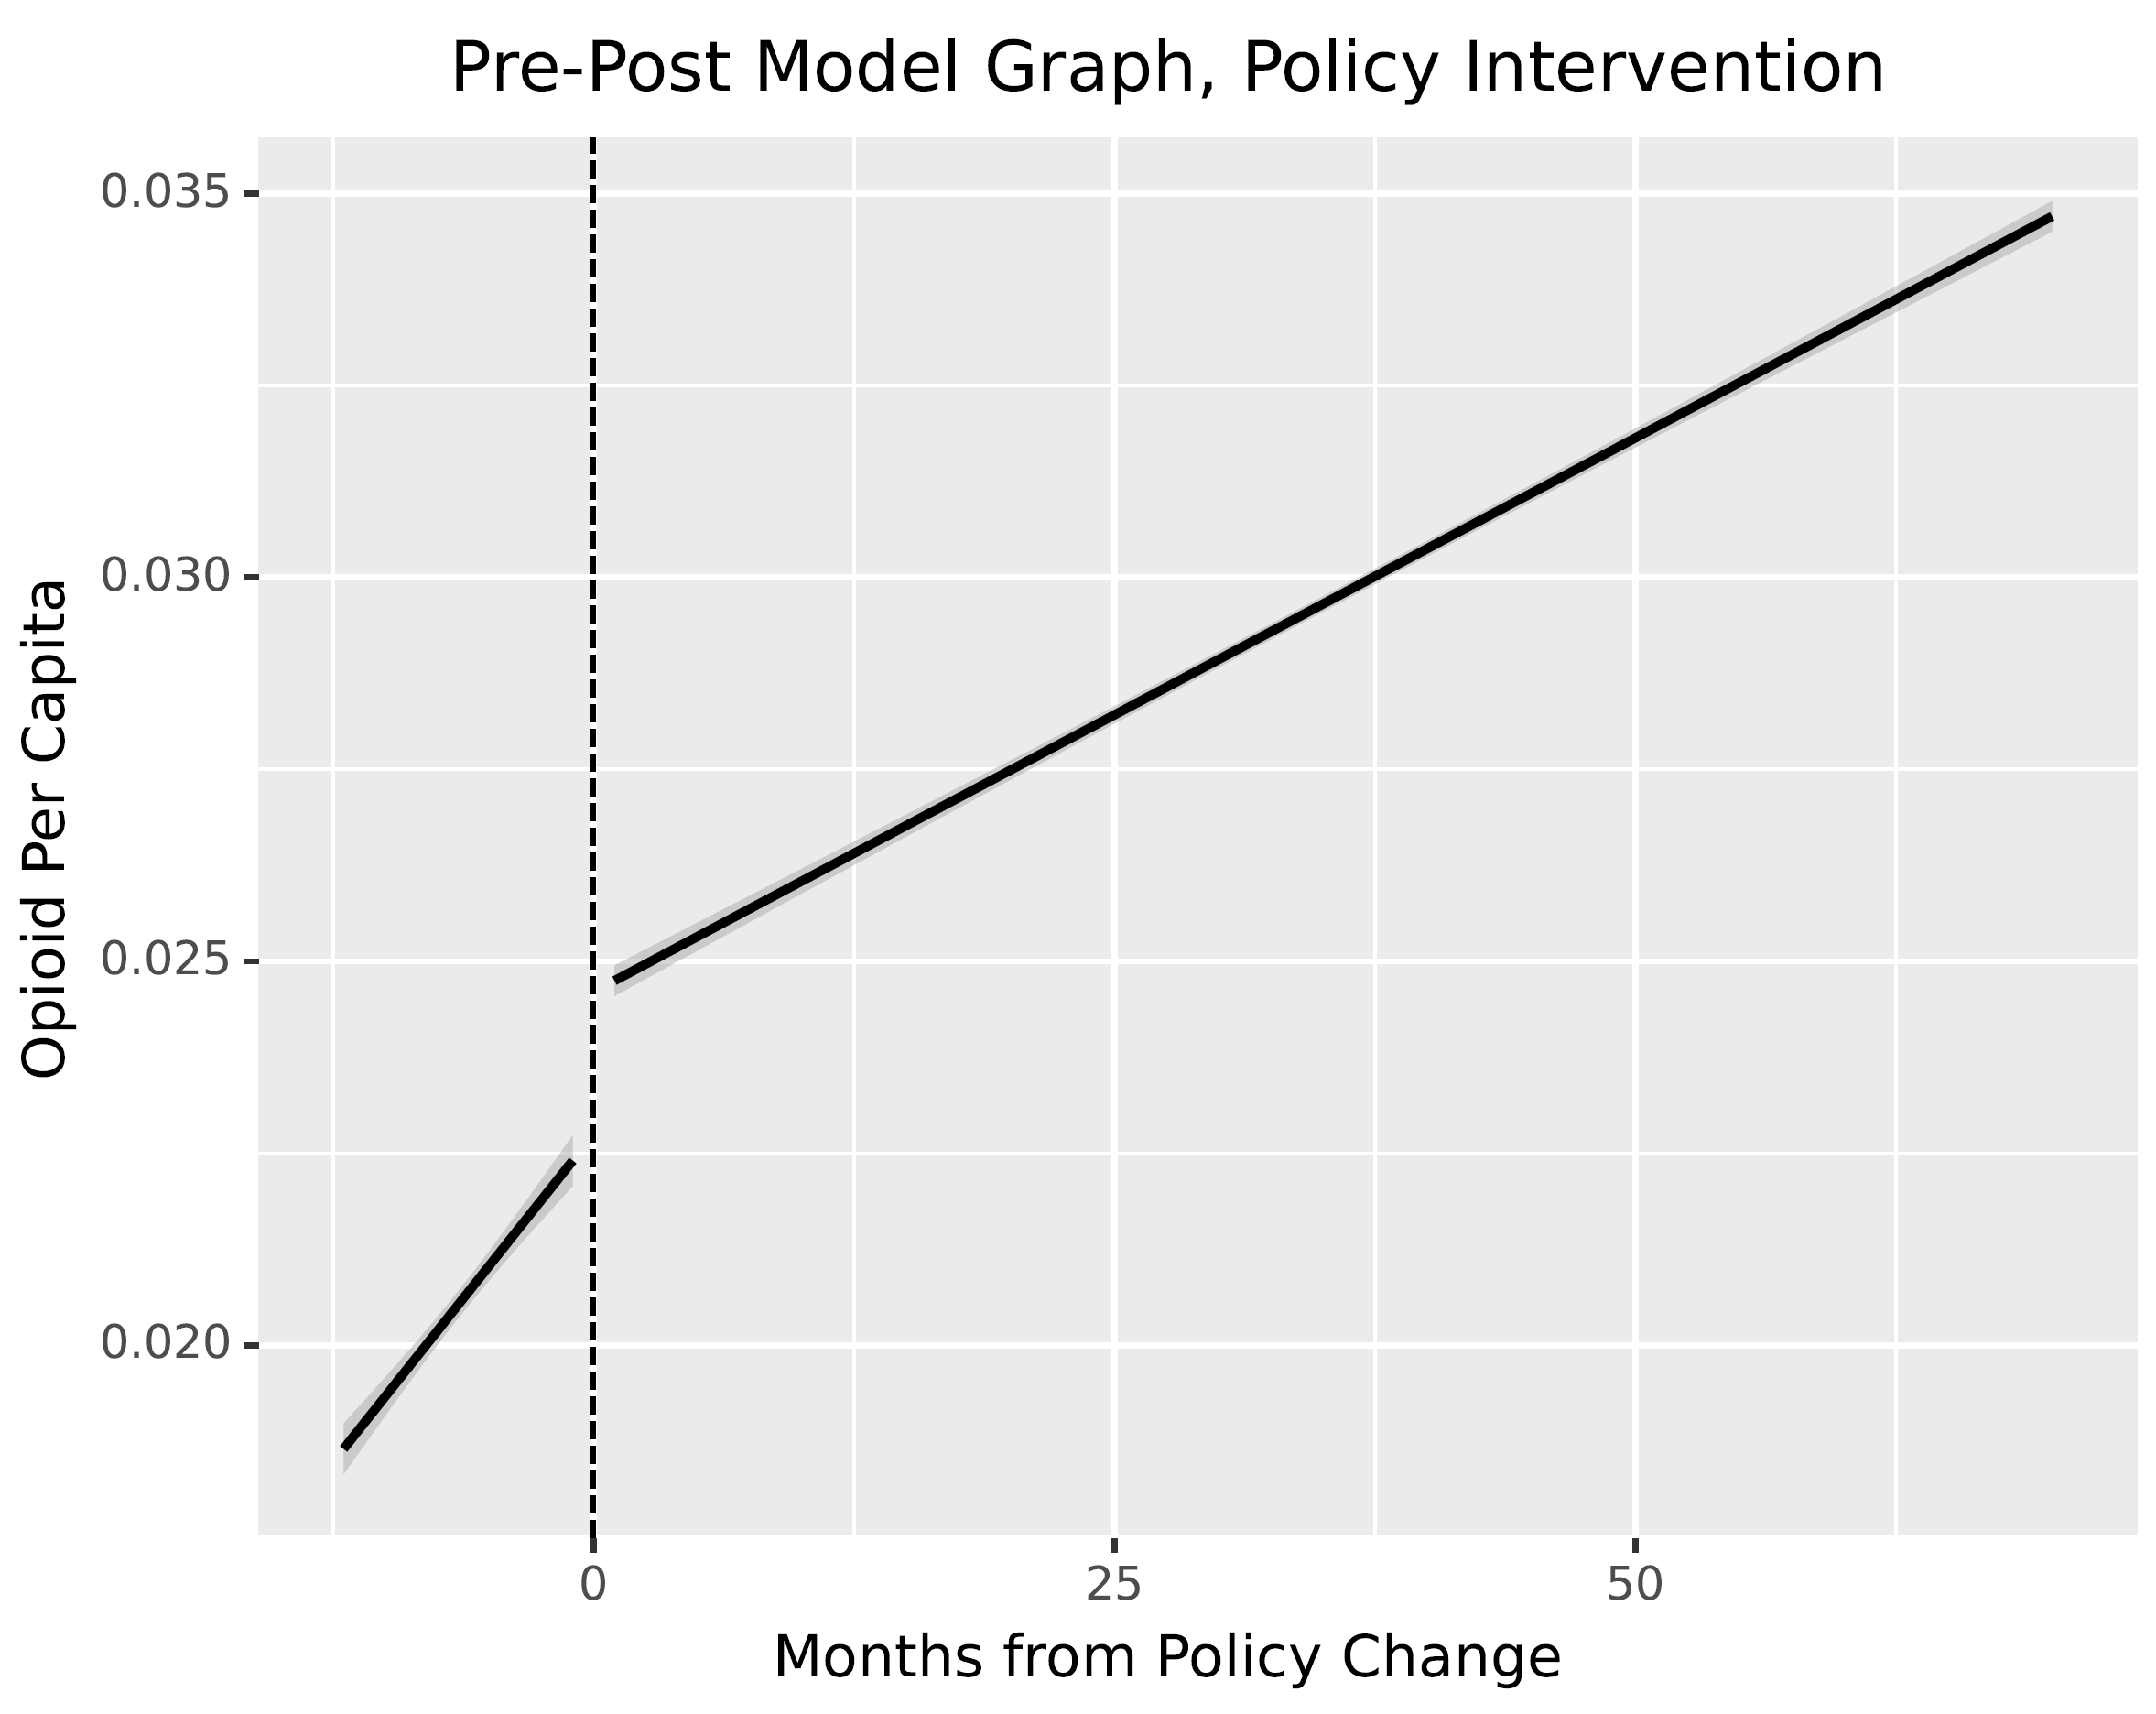
\includegraphics[width=0.7\linewidth]{../30_results/Bonus_Results/texas_opioid_shipment_prepost_monthly.png}
  \caption{Pre-post analysis}
  \label{fig:tx_ship_prepost}
\end{subfigure}%
\begin{subfigure}{.55\textwidth}
  \centering
  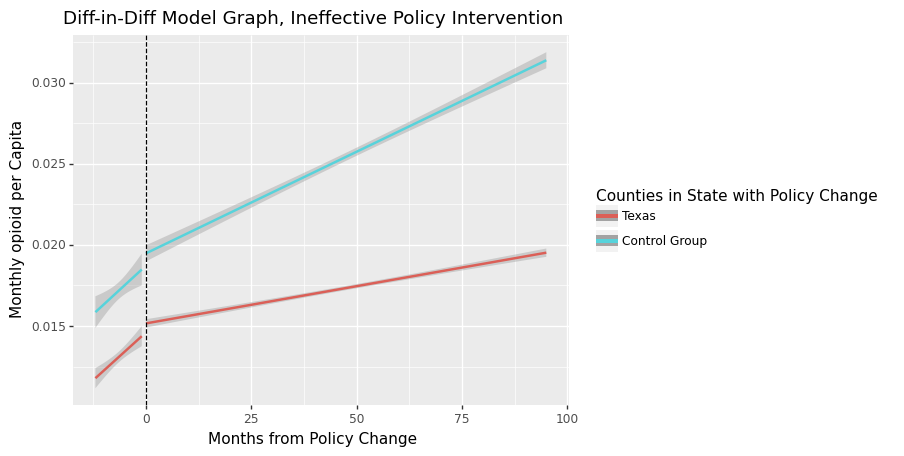
\includegraphics[width=1\linewidth]{../30_results/Bonus_Results/texas_opioid_shipment_diffdiff_monthly.png}
  \caption{Diff-in-diff analysis}
  \label{fig:tx_ship_did}
\end{subfigure}
\caption{Analysis of opioid policy on opioid shipments in Texas}
\floatfoot{\textit{Note:} The control group includes Mississippi, Montana, and Connecticut. The shipped opioids per capita are measured in grams and converted to morphine equivalents. The lines are the linear trend before and after the policy change. The shaded area indicates the range we expect our estimates to fall in with a 95\% level of confidence.}
\label{fig:tx_ship}
\end{figure}
Since the opioid shipment data is only available from 2006 on, meaning we only have one year of data before the policy change, we analyzed opioid shipment data by month instead of by year. The pre-post chart in Figure \ref{fig:tx_ship} shows an increasing trend in opioid shipments in Texas before and after the policy went into effect. However, the increase is less steep after the policy implementation in January 2007. Therefore, we may conclude that the policy restricted the opioid shipments by a small amount. For the difference-in-difference analysis, we selected Mississippi, Montana, and Connecticut as control groups. Before and after the policy implementation, the trend in Texas and the control states is positive. However, the increase in Texas is not as strong as in the control groups. Thus, we infer that the opioid policy in Texas successful in decreasing the rate of increase in opioid shipments. \\

\noindent \textbf{Overdose deaths}

\begin{figure}[!h]
\centering
\begin{subfigure}{.5\textwidth}
  \centering
  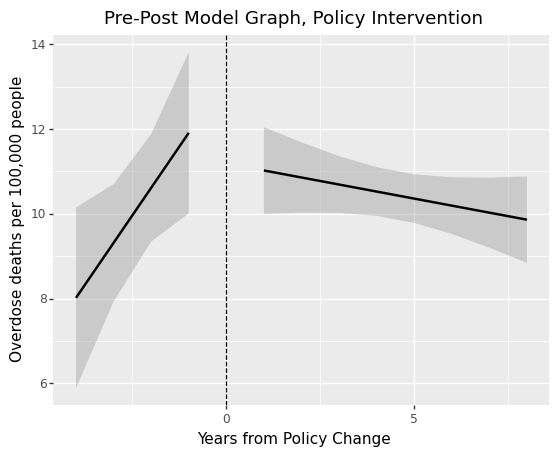
\includegraphics[width=0.7\linewidth]{../30_results/General_Results/texas_overdose_death_prepost.png}
  \caption{Pre-post analysis}
  \label{fig:tx_death_prepost}
\end{subfigure}%
\begin{subfigure}{.55\textwidth}
  \centering
  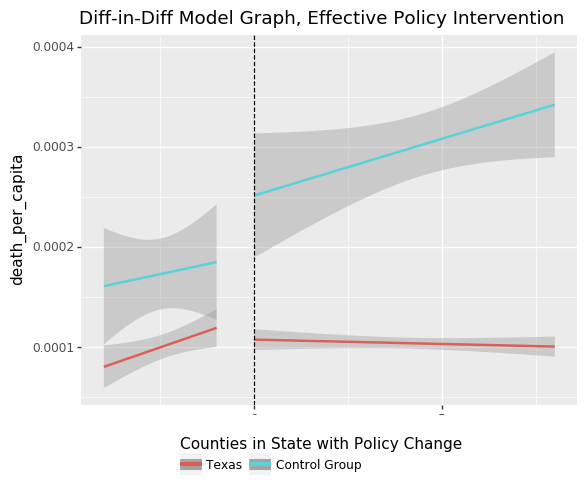
\includegraphics[width=1\linewidth]{../30_results/General_Results/texas_overdose_death_diffdiff.png}
  \caption{Diff-in-diff analysis}
  \label{fig:tx_death_did}
\end{subfigure}
\caption{Analysis of opioid policy on overdose deaths in Texas}
\floatfoot{\textit{Note:} The control group includes West Virginia, Oregon, and Idaho. The lines are the linear trend before and after the policy change. The shaded area indicates the range we expect our estimates to fall in with a 95\% level of confidence.}
\label{fig:tx_death}
\end{figure}

From the output of the pre-post graph, we can tell that the overdose deaths per 100,000 people increased year by year in Texas before the policy change and started to decrease annually after the policy's effective date. We selected West Virginia, Oregon, and Idaho as control states for the difference-in-difference analysis. It reveals that comparable without a policy change witness an increase in overdose deaths while Texas has a negative trend after the policy implementation. These results provide evidence that the decrease in overdose deaths per capita in Texas after 2007 is caused by the policy, which means that the policy is effective.

\subsection{Washington}
\textbf{Opioid shipments}

\begin{figure}[!h]
\centering
\begin{subfigure}{.5\textwidth}
  \centering
  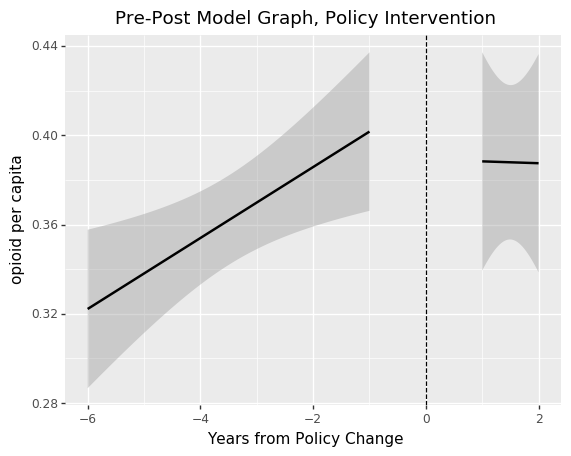
\includegraphics[width=0.7\linewidth]{../30_results/General_Results/washington_opioid_shipment_prepost.png}
  \caption{Pre-post analysis}
  \label{fig:wa_ship_prepost}
\end{subfigure}%
\begin{subfigure}{.55\textwidth}
  \centering
  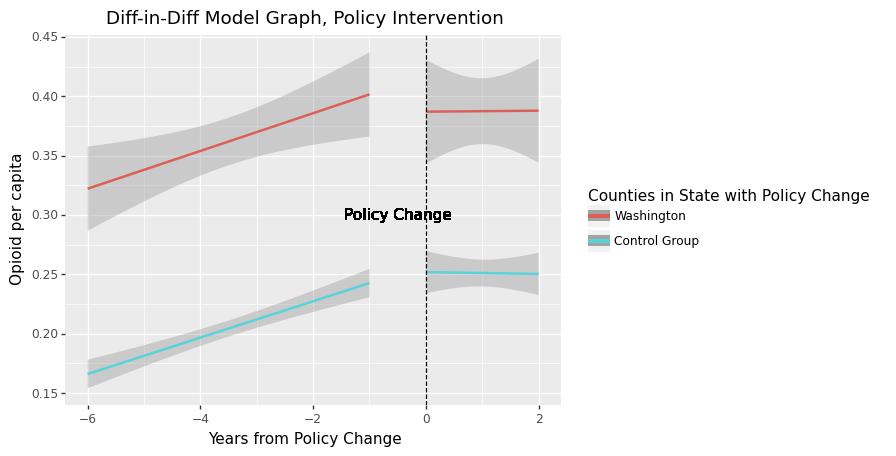
\includegraphics[width=1\linewidth]{../30_results/General_Results/washington_opioid_shipment_diffdiff.png}
  \caption{Diff-in-diff analysis}
  \label{fig:wa_ship_did}
\end{subfigure}
\caption{Analysis of opioid policy on opioid shipments in Washington}
\floatfoot{\textit{Note:} The control group includes Illinois, Wisconsin, and Rhode Islands. The shipped opioids per capita are measured in grams and converted to morphine equivalents. The lines are the linear trend before and after the policy change. The shaded area indicates the range we expect our estimates to fall in with a 95\% level of confidence.}
\label{fig:wa_ship}
\end{figure}

The pre-post analysis in Figure \ref{fig:wa_ship} indicates that there is a positive trend in opioid shipments in Washington before the policy is implemented. This trend changes after the policy went into effect in 2012 and is since then slightly negative. Even though the fall in opioid shipments is not very pronounced, the overall trend is totally different from the previous years. For the difference-in-difference analysis, we selected Illinois, Wisconsin, and Rhode Island as control groups. From the output, we can see that the development after the policy implementation is similar for Washington and the states in the control group. Hence, the pre-post analysis and the diff-in-diff analysis provide opposing conclusion. Due to the statistical superiority of the latter, we cannot conclude that the policy is successful in Washington with regards to shipped opioids. \\

\noindent \textbf{Overdose deaths}

\begin{figure}[!h]
\centering
\begin{subfigure}{.5\textwidth}
  \centering
  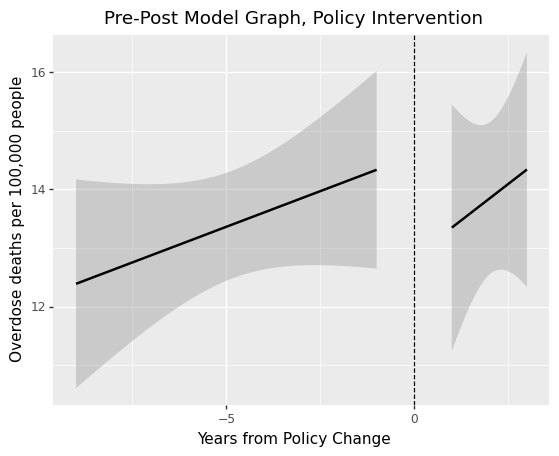
\includegraphics[width=0.7\linewidth]{../30_results/General_Results/washington_overdose_death_prepost.png}
  \caption{Pre-post analysis}
  \label{fig:wa_death_prepost}
\end{subfigure}%
\begin{subfigure}{.55\textwidth}
  \centering
  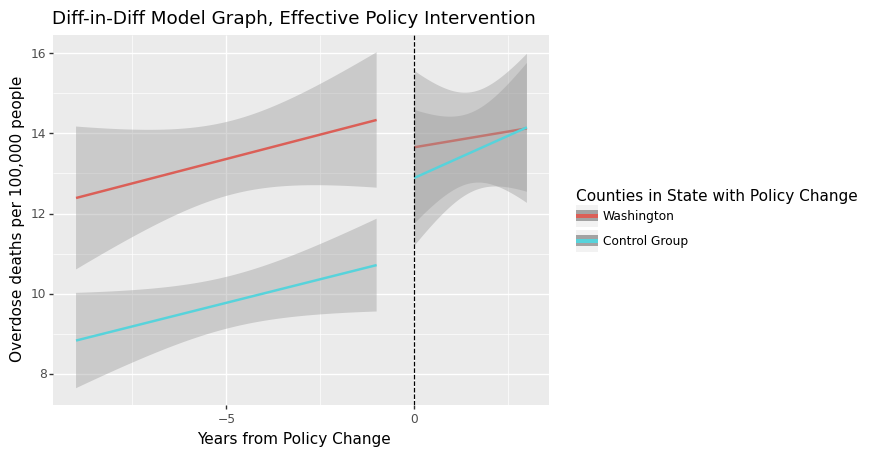
\includegraphics[width=1\linewidth]{../30_results/General_Results/washington_overdose_death_diffdiff.png}
  \caption{Diff-in-diff analysis}
  \label{fig:wa_death_did}
\end{subfigure}
\caption{Analysis of opioid policy on overdose deaths in Washington}
\floatfoot{\textit{Note:} The control group includes Kansas, New Jersey, and Oregon. The lines are the linear trend before and after the policy change. The shaded area indicates the range we expect our estimates to fall in with a 95\% level of confidence.}
\label{fig:wa_death}
\end{figure}

From the pre-post graph in Figure \ref{fig:wa_death}, we can tell that the number of overdose deaths per 100,000 people in Washington was both increasing before and after the policy became effective. Though briefly after the policy implementation, the overdose deaths per capita became lower, they still increased year by year after the policy's effective date by an even larger number. Combining this insight with the output from the difference-in-difference analysis, we can see that the trends for both Washington and states in the control group are the same before the policy became effective. After that, the increase in Washington is lower than in the control group which consists of Kansas, New Jersey, and Oregon. Therefore, we can conclude that the policy was not successful in reducing the absolute overdose death numbers. However, it achieved to control the increasing trend of overdose deaths in Washington compared to similar states.

\section{Limitations}

The first limitation of our analysis is that since the US census population data is published once every decade, the population data except for 2010 are estimated. The exact population could be different from the data we used in our analysis. Also, since we used monthly opioid shipment data instead of yearly data but used yearly populations instead of monthly populations at the same time to analyze the effect of policy on opioid shipment in Texas, our analysis may not fully reflect the real situation. However, we assume that population won’t change dramatically, hence, the trend should be the same. Thirdly, in the difference-in-differences analysis, we selected states that are similar in terms of how their opioid shipments and deaths are trending over time before the policy went into effect. Besides that, we only selected three states as comparison states for every one of those states that had drug control policies. However, factors like income, population, etc., should also be taken into account. In addition, these comparison states may also have had some regulatory guidelines that were not implemented by the law but also impacted both the shipment and overdose deaths of opioids.
Lastly, we do not have overdose death available for counties with less than 10 deaths per year per category. For that reason, we cannot account for the effects of the policy in these low overdose death counties.


\section{Conclusion}


Based on the graphs of our pre-post and difference-in-difference analysis, Florida's drug policy was effective in decreasing the prescription opioid shipment amount as well as decreasing the overdose deaths. Texas' drug policy decreased the rate of increase in opioid shipments and did change the trend in overdose deaths from increasing to decreasing. In contrast, Washington's drug policy was not successful in controlling the opioid shipments. It only lowered the still increasing rate of overdose deaths compared to similar states.

By comparing policies in the three states, we can learn that since there were a series of changes in Florida that strictly prohibited physician dispensing of drugs and penalized it by arrest, seizure of assets, and clinic closure, strict policies combined with the practical implementation of penalties achieve that the policy has the desired effect. However, policies in both Texas and Washington were mainly focused on performing patient evaluation and consulting, obtaining patients' consent, and making dose recommendations. These policies seem to be too moderate to be very effective, and in the meantime, no severe penalty was introduced. Furthermore, policies in Florida focused on cutting off the source of prescription opioids, which reduced opioid dispensing to the greatest extent possible. To sum up, the problem's root cause should be considered when making policies, and strict rules that are well-applied can assist in producing the intended effects.


\end{document}
